
\author{Anders Eiler}
\section{Design}
\subsection{What we already know}
\begin{frame}{Design}
  \begin{block}{What we already know}
  \begin{itemize}
  	\item One master-server.
  	\item One slave-server per drone. Many drones. 
  \end{itemize}

  \begin{figure}[htb]
    \centering
    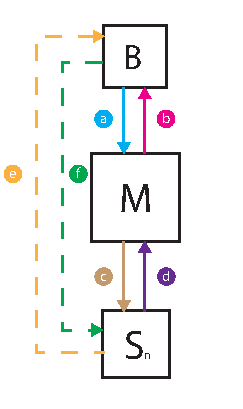
\includegraphics[width=0.25\textwidth]{gfx/dataflow_diagram.pdf}
    \caption{Dataflow diagram}
  \end{figure}

  \end{block}
\end{frame}

\subsection{Privileges}
\begin{frame}{Privileges}{Design}
  \begin{block}{}
  	There are three ways of assigning privileges to many users:

  	\begin{itemize}
  		\item Each privilege to each user.
  	\end{itemize}

  	\begin{align}
		I_1 = |U|*|P|
	\end{align}
  \end{block}
\end{frame}

\begin{frame}{Privileges}{Design}
  \begin{block}{}
  	\begin{itemize}
  		\item Privileges added to roles, users to roles and exceptions to users.
  	\end{itemize}

	\begin{align}
		I_{rm} = |U| - |u_{m}| + |P| + \sum_{i \in u_{m}} |P|-|p_{m}(i)|
	\end{align}
  \end{block}
\end{frame}

\begin{frame}{Privileges}{Design}
  \begin{block}{}
  	\begin{itemize}
  		\item Lowest denominator of privileges added to roles, extra privileges added to users.
  	\end{itemize}
  	
	\begin{align}
		I_{lcd} = \left|p_{lcd}\left(U\right)\right| + \left|U\right| + \sum_{i \in U} \left|p\left(i\right)\right|\textbackslash\left|p_{lcd}\left(U\right)\right|
	\end{align}
  \end{block}
\end{frame}

\begin{frame}{Privileges}{Design}
  \begin{block}{}
  	\begin{itemize}
  		\item LONE supports all three privilege organization types.
  		\item Tradeoff:
  		\begin{itemize}
  			\item Either it uses a lot of space, is expensive to write and cheap to read.
  			\item Or it is space-efficient and expensive to read. 
  		\end{itemize}
  		\item The choice depends on the use-case of LONE!
  	\end{itemize}
  \end{block}
\end{frame}



\subsection{The number of slaves per drone}
\begin{frame}{The number of slaves per drone}{Design}
  \begin{block}{How many slaves per drone, or drones per slave?}
	The current design uses one slave per drone. Is this the right design?

	Potential issues:
	\begin{itemize}
		\item Hardware overflow -- too much hardware on systems with low load.
		\item Too little hardware on systems with high load.
	\end{itemize}

	Solution?
  \end{block}
\end{frame}



\subsection{Rails Sessions - User Authentication}
\begin{frame}{Rails Sessions - User Authentication}{Design}
  \begin{block}{Who is that?}
  	How do you tell users apart? We use unique identifiers, passwords and sessions. \\

  	Ruby on Rails provides a lot of tools to enhance the security when using sessions such as:
  	\begin{itemize}
  		\item Session ID
  		\item Protection against Session Hijacking
  		\item Safe Session storage
  	\end{itemize}
  \end{block}
\end{frame}


\subsection{Design outlines and decisions}
\begin{frame}{Design outlines and decisions}{Design}
  \begin{block}{Maintainability}
  	\begin{itemize}
  		\item Easy to administrate the system.
  		\item Easy to maintain the code.
  	\end{itemize}
  \end{block}

  \begin{block}{Scalability}
  	\begin{itemize}
  		\item Addition of new slaves, users and privileges.
  		\item Addition of new types of equipment.
  	\end{itemize}
  \end{block}
\end{frame}

